% ============================================================================
% Deliverable 1 - Generative Artificial Intelligence (580694), Primavera 2026
% Universidad de Concepcion  --  version en espanol
% Poster / resumen ejecutivo de UNA pagina.
% Compilar:  pdflatex deliverable1_es.tex   (ejecutar dos veces)
% ============================================================================
\documentclass[9pt,a4paper]{extarticle}

\usepackage[utf8]{inputenc}
\usepackage[T1]{fontenc}
\usepackage[margin=0.8cm,top=0.6cm,bottom=0.35cm]{geometry}
\usepackage{helvet}\renewcommand{\familydefault}{\sfdefault}
\usepackage{xcolor}
\usepackage{multicol}
\usepackage{booktabs}
\usepackage{enumitem}
\usepackage{tcolorbox}
\usepackage{pgfplots}
\usepackage{microtype}
\pgfplotsset{compat=1.16}
\tcbuselibrary{skins}

% sin patrones de silabacion en espanol instalados: evitamos partir palabras
\hyphenpenalty=10000 \exhyphenpenalty=10000 \tolerance=3000 \emergencystretch=2.5em

% ---------------------------------------------------------------- paleta ---
% Paleta sobria de dos tonos frios (navy/steel) + un acento calido discreto
% (bronce apagado) para separadores, y un rojo apagado reservado solo para
% datos negativos/criticos (nunca decorativo).
\definecolor{navy}{HTML}{1E2A3A}
\definecolor{steel}{HTML}{5B6B7C}
\definecolor{amber}{HTML}{8C7A5B}
\definecolor{crimson}{HTML}{8C3B3B}
\definecolor{paper}{HTML}{F4F4F2}
\definecolor{rule}{HTML}{D6D8DB}
\definecolor{note}{HTML}{ECEEF0}

\setlength{\parindent}{0pt}
\setlength{\columnsep}{6.5mm}
\setlength{\multicolsep}{2pt}
\setlength{\parskip}{0.5mm}
\pagestyle{empty}

% --------------------------------------------------------------- ayudas ----
\newcommand{\heading}[1]{%
  \par\vspace{1.1mm}\noindent
  {\color{navy}\bfseries\small\MakeUppercase{#1}}
  \par\vspace{0.7mm}\noindent
  {\color{amber}\rule{\linewidth}{1.1pt}}
  \par\vspace{0.6mm}\noindent\ignorespaces}

\newtcolorbox{keybox}[1]{colback=note,colframe=amber,boxrule=0.8pt,
  left=2mm,right=2mm,top=1.5mm,bottom=1.5mm,arc=1mm,
  fonttitle=\bfseries\footnotesize,coltitle=white,colbacktitle=amber,title={#1}}

\newtcolorbox{quietbox}{colback=paper,colframe=rule,boxrule=0.5pt,
  left=2mm,right=2mm,top=1.5mm,bottom=1.5mm,arc=1mm}

\newcommand{\ph}[1]{\colorbox{note}{\textcolor{navy}{\textbf{#1}}}}
\setlist[itemize]{leftmargin=3.6mm,itemsep=0.55mm,topsep=0.75mm,parsep=0pt}

\begin{document}
\small

% ================================================================ CABECERA ==
\begin{tcolorbox}[colback=navy,colframe=navy,boxrule=0pt,left=3mm,right=3mm,
                  top=2mm,bottom=2mm,arc=1mm]
{\color{white}\bfseries\LARGE Modelos de lenguaje peque\~nos para decidir en combate en Pok\'emon Blue}\\[1.1mm]
{\color{white!85}\large El prompting estructurado arregla el formato de la acci\'on, no la calidad de la decisi\'on}\\[2mm]
{\color{white!75}\footnotesize
Deliverable 1 \ \textbullet\ \ Generative Artificial Intelligence (580694), Primavera 2026 \ \textbullet\ \ Universidad de Concepci\'on}\\[1.4mm]
{\footnotesize\color{white!85}Equipo:} \ph{Nombre 1 \textbullet\ Nombre 2 \textbullet\ Nombre 3 \textbullet\ Nombre 4}
\hfill
{\footnotesize\color{white!85}Repositorio:} \ph{github.com/usuario/repositorio}
\end{tcolorbox}

\vspace{1.5mm}
\begin{multicols}{2}

% ========================================================== 1. LA TAREA =====
\heading{1. Especificaci\'on de la tarea}
El modelo act\'ua como \textbf{m\'odulo de decisi\'on de combate} de un agente de Pok\'emon Blue.

\textbf{Entrada.} Estado de combate estructurado: tipo(s), \%\ de HP y velocidad de ambos Pok\'emon, m\'as los cuatro movimientos con \emph{nombre, tipo, potencia, precisi\'on} y \emph{PP restantes}.

\textbf{Salida.} Exactamente una etiqueta ejecutable: \texttt{MOVE\_1}, \texttt{MOVE\_2}, \texttt{MOVE\_3} o \texttt{MOVE\_4}.

\textbf{Qu\'e cuenta como correcto.} La etiqueta que maximiza una pol\'itica ofensiva expl\'icita y determinista,
\par\vspace{0.6mm}\noindent\hspace*{\fill}%
\colorbox{paper}{\;\texttt{score = potencia $\times$ precisi\'on $\times$ STAB $\times$ efectividad}\;}%
\hspace*{\fill}\par\vspace{0.8mm}\noindent
con \texttt{score = 0} cuando \texttt{PP = 0}: ground truth reproducible y auditable caso por caso.

\textbf{Por qu\'e no es trivial.} Los cinco atributos compiten: el movimiento de mayor potencia es el \'optimo en solo 19 de 30 estados, y las inmunidades de Gen~I (El\'ectrico\,$\to$\,Tierra, Normal\,$\to$\,Fantasma) anulan la opci\'on que parece m\'as fuerte. El modelo debe \emph{combinar} restricciones, no recuperar un dato.

% ======================================================= 2. PILOTO =========
\heading{2. Experimento piloto (v1)}
\textbf{Modelo.} Qwen2.5-1.5B-Instruct, decodificaci\'on greedy, \texttt{max\_new\_tokens=48}, semilla \texttt{20260830}, mismo system prompt en ambas condiciones.

\textbf{Dise\~no.} 30 estados sint\'eticos (10 EASY / 10 MEDIUM / 10 HARD, seg\'un la raz\'on entre el mejor y el segundo mejor score: $\geq$1,80 / 1,25--1,80 / 1,01--1,25). \textbf{Los mismos 30 estados} van a los dos prompts $\rightarrow$ \textbf{60 inferencias}, offline y sin el emulador en la medici\'on.

\textbf{Condiciones.} \textsc{Direct} = petici\'on natural (``What move would you use next?''). \textsc{Structured} = mismo estado, checklist de razonamiento y contrato de salida estricto (solo \texttt{MOVE\_N}).

\textbf{M\'etricas.} \textsc{Strict} (responde exactamente \texttt{MOVE\_N} y es ejecutable) $\cdot$ \textsc{Interp} (intenci\'on recuperable) $\cdot$ \textsc{Acc} (coincide con el ground truth) $\cdot$ \emph{regret} (mejor score perdido).

\vspace{0.8mm}
{\centering
\begin{tabular}{@{}lrrrr@{}}
\toprule
\textbf{Prompt} & \textsc{Strict} & \textsc{Interp} & \textsc{Acc} & \textsc{Exec-c.}\\
\midrule
\textsc{Direct}     & 0,0\,\%  & 36,7\,\% & 3,3\,\%  & 0,0\,\%\\
\textsc{Structured} & \textbf{96,7\,\%} & \textbf{96,7\,\%} & \textcolor{crimson}{\textbf{16,7\,\%}} & 16,7\,\%\\
\bottomrule
\end{tabular}\par}
\vspace{0.4mm}
{\footnotesize \emph{Regret} medio: \textsc{Direct} 0,41; \textsc{Structured} 0,49. $n=30$ estados por condici\'on.}

% ==================================================== 3. DIAGNOSTICO =======
\heading{3. Diagn\'ostico del fallo}
El prompting estructurado \emph{casi elimin\'o} el problema de interfaz (\textsc{Strict} $0\,\%\rightarrow$ 96,7\,\%; una respuesta sigui\'o siendo inejecutable), as\'i que el agente ya puede ejecutarse solo. No resolvi\'o la tarea: la calidad de la decisi\'on queda \textbf{por debajo del azar}.

\textbf{El modelo responde por posici\'on, no por estado.} En las 29 respuestas parseables devuelve \texttt{MOVE\_2} veinte veces y \texttt{MOVE\_1} \emph{ninguna}, mientras que la acci\'on \'optima est\'a repartida casi uniformemente entre las cuatro posiciones ($\chi^2(3)=31{,}8$; $p<10^{-6}$ frente a la uniforme).

\vspace{0.5mm}
{\centering
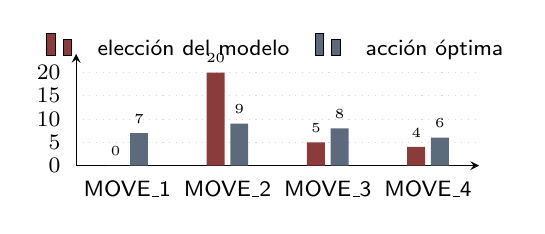
\begin{tikzpicture}
\begin{axis}[
  width=6.7cm, height=3.0cm, ybar, bar width=6.5pt, ymin=0, ymax=24,
  symbolic x coords={MOVE\_1,MOVE\_2,MOVE\_3,MOVE\_4},
  xtick=data, xticklabel style={font=\footnotesize},
  yticklabel style={font=\footnotesize}, ytick={0,5,10,15,20},
  legend style={font=\footnotesize,at={(0.5,1.24)},anchor=north,legend columns=2,
                draw=none,fill=none,column sep=2.5mm},
  axis lines=left, tick style={draw=none},
  ymajorgrids, grid style={rule,dotted},
  enlarge x limits=0.17, nodes near coords,
  every node near coord/.append style={font=\tiny}]
\addplot[fill=crimson,draw=none] coordinates {(MOVE\_1,0)(MOVE\_2,20)(MOVE\_3,5)(MOVE\_4,4)};
\addplot[fill=steel,draw=none]   coordinates {(MOVE\_1,7)(MOVE\_2,9)(MOVE\_3,8)(MOVE\_4,6)};
\legend{elecci\'on del modelo, acci\'on \'optima}
\end{axis}
\end{tikzpicture}\par}
\vspace{-0.5mm}

\textbf{Solo acierta cuando la respuesta resulta ser \texttt{MOVE\_2}.} Tasa de acierto seg\'un la posici\'on del movimiento \'optimo: \texttt{MOVE\_1} \textbf{0/7}, \texttt{MOVE\_2} 4/9, \texttt{MOVE\_3} 1/8, \texttt{MOVE\_4} \textbf{0/6}.

\vspace{0.6mm}

{\centering
\begin{tabular}{@{}lr@{}}
\toprule
\textbf{Pol\'itica} & \textbf{Exactitud}\\
\midrule
Qwen2.5-1.5B, prompt estructurado   & \textcolor{crimson}{\textbf{16,7\,\%}}\\
Elecci\'on aleatoria uniforme (4 opciones) & 25,0\,\%\\
Pol\'itica constante ``siempre \texttt{MOVE\_2}'' & 30,0\,\%\\
$\max$(potencia $\times$ precisi\'on), PP\,$>$\,0 & 53,3\,\%\\
$\max$(potencia) --- ignora los tipos & \textbf{63,3\,\%}\\
\bottomrule
\end{tabular}\par}
\vspace{1.4mm}

\begin{keybox}{Diagn\'ostico}
El principal cuello de botella observado \textbf{no} es el formato de salida, sino la \textbf{selecci\'on de acciones al combinar m\'ultiples restricciones}: al ponderar efectividad, STAB, potencia, precisi\'on y PP sobre cuatro candidatos a la vez, el modelo colapsa en un \textbf{sesgo de posici\'on} casi independiente del estado. Una heur\'istica de una l\'inea que ignora la tabla de tipos es \textbf{3,8 veces} m\'as precisa.
\end{keybox}

% =================================================== 4. VALIDEZ GT =========
\heading{4. \textmd{\bfseries ¿}Es el ground truth el problema?}
Una puntuaci\'on baja frente a una pol\'itica hecha a mano podr\'ia significar que la pol\'itica est\'a mal. Tres comprobaciones lo descartan: son errores indefendibles bajo \emph{cualquier} regla.
\begin{itemize}
\item \textbf{Movimiento sin efecto.} Caso 16 (abajo): \emph{Thunderbolt} (El\'ectrico) contra un rival \textbf{Tierra} --- inmune, 0 de da\~no.
\item \textbf{Movimiento inejecutable.} Caso 29: eligi\'o un movimiento con \textbf{PP = 0}; el agente no puede emitirlo.
\item \textbf{Peor opci\'on estricta} elegida en \textbf{6 de 29} respuestas (21\,\%): la de menor score de las cuatro.
\end{itemize}

\vspace{-0.5mm}
\begin{quietbox}
{\footnotesize\ttfamily
CASO 16 -- jugador Flying (41\% HP) vs Ground (53\%)\\[0.4mm]
MOVE\_1 Psybeam\ \ \ \ Psychic\ \ P65 A100 \ \ score 65,0\\
MOVE\_2 Thunderbolt Electric P95 A100 \ \ score \ \textcolor{crimson}{\textbf{0,0}}\\
MOVE\_3 Rock Throw\ \ Rock\ \ \ \ \ P50 \ A65 \ \ score 16,3\\
MOVE\_4 Ember\ \ \ \ \ \ Fire\ \ \ \ \ P40 A100 \ \ score 40,0\\[0.6mm]
ground truth = MOVE\_1 \ \ \ \ modelo = \textcolor{crimson}{\textbf{MOVE\_2}}}\\[0.6mm]
{\footnotesize Se queda con el n\'umero de potencia m\'as alto e ignora la inmunidad que lo vuelve in\'util.}
\end{quietbox}

\textbf{Sin gradiente de dificultad.} La exactitud estructurada es EASY 2/10, MEDIUM 1/10, HARD 2/10. Un razonamiento graduado deber\'ia degradarse al subir la dificultad; un sesgo de posici\'on no --- y no lo hace.

% ======================================================= 5. AMENAZAS ======
\heading{5. Amenazas a la validez y correcci\'on para la v2}
\begin{itemize}
\item \textbf{T1.} A \textsc{Direct} nunca se le pidi\'o \texttt{MOVE\_N}, as\'i que su $0\,\%$ de \textsc{Strict} es cierto por construcci\'on; se reporta como l\'inea base de interfaz, no como evidencia de razonamiento.
\item \textbf{T2.} \texttt{max\_new\_tokens=48} trunc\'o las respuestas libres de \textsc{Direct} y desinfla su 36,7\,\% de \textsc{Interp}.
\item \textbf{T3.} La pol\'itica de referencia es solo ofensiva: no cubre movimientos de estado, cambios, objetos ni varios turnos.
\end{itemize}
\textbf{v2.} Ambos prompts exigen el mismo contrato \texttt{MOVE\_N}, as\'i la \'unica diferencia es el andamiaje de razonamiento; $n=50$ estados, cada uno repetido con sus movimientos \textbf{permutados}, lo que mide el sesgo de posici\'on de forma directa.

% ==================================================== 6. MODELOS ==========
\heading{6. Modelos propuestos (todos muy por debajo de 8B)}
{\centering
\begin{tabular}{@{}lrrrrr@{}}
\toprule
\textbf{Modelo} & \textbf{Par.} & \textbf{MMLU} & \textbf{IFEval} & \textbf{GSM8K} & \textbf{fp16}\\
\midrule
Qwen2.5-1.5B-Instr. & 1,5B & 50,7 & 42,5 & 73,2 & 3,1\,GB\\
Llama-3.2-3B-Instr. & 3,2B & 63,4 & \textbf{77,4} & 77,7 & 6,4\,GB\\
Phi-3.5-mini-instr. & 3,8B & \textbf{69,0} & n.r. & \textbf{86,2} & 7,6\,GB\\
\bottomrule
\end{tabular}\par}
\vspace{0.3mm}
{\footnotesize Fuentes: fichas oficiales de Qwen2.5, Llama 3.2 y Phi-3.5-mini (referencias en el repositorio). Los protocolos difieren, as\'i que ubican a los modelos en una clase m\'as que ordenarlos. n.r. = no reportado.}
\vspace{0.6mm}

\begin{itemize}
\item \textbf{IFEval: seguimiento de instrucciones.} Mide obediencia a formatos restringidos, que es lo que necesita el controlador. Con el prompt estructurado Qwen ya alcanza 96,7\,\% pese a su 42,5, as\'i que el formato \emph{no} es lo que separa a los candidatos.
\item \textbf{GSM8K: razonamiento de varios pasos.} Proxy p\'ublico m\'as cercano al paso que s\'i falla: combinar varios atributos num\'ericos. Phi-3.5-mini lidera con \textbf{86,2} usando solo 3,8B: la prueba directa de si ese cuello de botella se levanta.
\end{itemize}
Qwen2.5-1.5B es adem\'as la l\'inea base: el \'unico con un perfil \emph{medido} aqu\'i. La tarea no exige de forma evidente un modelo de 8B, lo que motiva evaluar candidatos bastante m\'as peque\~nos; el mayor es de \textbf{3,8B}.

\end{multicols}

\vspace{-2mm}
\begin{tcolorbox}[colback=paper,colframe=navy,boxrule=0.9pt,left=2.5mm,right=2.5mm,
                  top=1.2mm,bottom=1.2mm,arc=1mm,
                  fonttitle=\bfseries\footnotesize,coltitle=white,colbacktitle=navy,
                  title={7. VIABILIDAD DE EJECUCI\'ON Y REPRODUCIBILIDAD}]
\footnotesize
El piloto \textbf{ya se ejecut\'o de principio a fin} en el hardware del equipo: 60 inferencias, \textbf{105,5 min} en \textbf{CPU}, de forma determinista (greedy, semilla fija). Memoria estimada como par\'ametros $\times$ 2 bytes (fp16) m\'as cach\'e KV: los tres caben en una Colab T4 gratuita (16\,GB). El repositorio incluye el benchmark, sus cuatro archivos de resultados y la demo en PyBoy, que se mantiene \emph{fuera} del circuito de medici\'on para no confundir errores del emulador con fallos del modelo.
\end{tcolorbox}

\end{document}
